\documentclass[a4paper,10pt,twocolumn,uplatex]{jsarticle}
\usepackage{style/nislab,style/resume}

%---------------------------------------------------------------------
% レジュメ種別・日付設定(要変更)
% \type{} 1:修士論文諮問会 2:卒業論文発表会 3:月例発表会 4:研究室合同発表会
%---------------------------------------------------------------------
\type{3}
\year{2021}
\month{10}
\date{9}

%---------------------------------------------------------------------
% ページ番号設定(要変更)
%---------------------------------------------------------------------
\setcounter{page}{5}
%---------------------------------------------------------------------
% 変更不要
%---------------------------------------------------------------------
\begin{document}

%---------------------------------------------------------------------
% タイトル作成部分(要変更)
% \maketitle{タイトル}{title}{名前}{name}
%---------------------------------------------------------------------
\maketitle{ホームネットワークにおけるSDNによる仮想デバイスを用いた\\セキュリティプラットフォームの検討}
{A Study of SDN-based Security Platform for Home Networks}
{塚﨑 拓真}
{Takuma Tsukasaki}

%---------------------------------------------------------------------
\section{はじめに}
近年,IoT(Internet of Things)が注目を集めるようになり,今後あらゆるモノがネットワークに接続され,利用されることが予想される.
それに伴い,ネットワーク内には様々な端末や機器(まとめて,デバイス)が混在することになり,ホームネットワークの形態は多様化していくと考えられる.\par
しかし,IoTの発展で利便性が高まる一方で,これまでネットワークに接続されていなかったモノが接続されることにより,セキュリティ上のリスクも高まっている\cite{guideline}.
IoTデバイスは十分なセキュリティを考慮せずに開発されたものが多いため,悪意のある攻撃者によるサイバー攻撃の標的になりやすい.
セキュリティ上の脅威が各種デバイスに顕在した場合,個別に対処するとコストや時間がかかってしまうため,脅威に対し一括に対処する必要がある.
しかし,ホームネットワーク内には異なる規格のハードウェアや様々なアプリケーションが混在しているため,それら全てに対応したシステムの構築や更新を続けるのは困難である.
そのため,ホームネットワーク内で通信するのであれば,どのデバイスも必ず利用するネットワークを利用したシステムを構築することが望ましい.本研究では,SDNを用いて,ホームネットワークに適した形での不正な通信の検知を検討する.

%---------------------------------------------------------------------
\section{関連研究}
今野らは,セキュリティ対策を施し,仮想的に作成した論理デバイスを利用し,実際のIoTデバイスの通信を中継することで,セキュアな通信環境を提供するプラットフォームを提案した\cite{logic}.これにより,IoTデバイスのリソース量に依存しないセキュリティ対策の実現が可能となる.しかし,クラウドサーバ宛て,ローカルネットワーク上のサーバ宛ての2パターンを前提としている.現在のスマートホームデバイスは,クラウド上のシステムと連携することで,デバイス間の連携を可能にしているが,今後はホームネットワーク内で閉じたデバイス間の通信によって連携を行う形になることが想定される\cite{d2d}.デバイス間で直接通信を行う場合,各デバイスでどういったデバイスとの通信を受け入れるか,アクセス制御を行う必要がある.しかし,全てのデバイスがアクセス制御に対応しているとは限らず,デバイスの計算能力の制限によって実現できるアクセス制御に制限があったり,デバイスのソフトウェア自体の脆弱性によってアクセス制御が機能しない場合が考えられる\cite{disap}.

%---------------------------------------------------------------------
\begin{figure}[!tb]
  \centering
  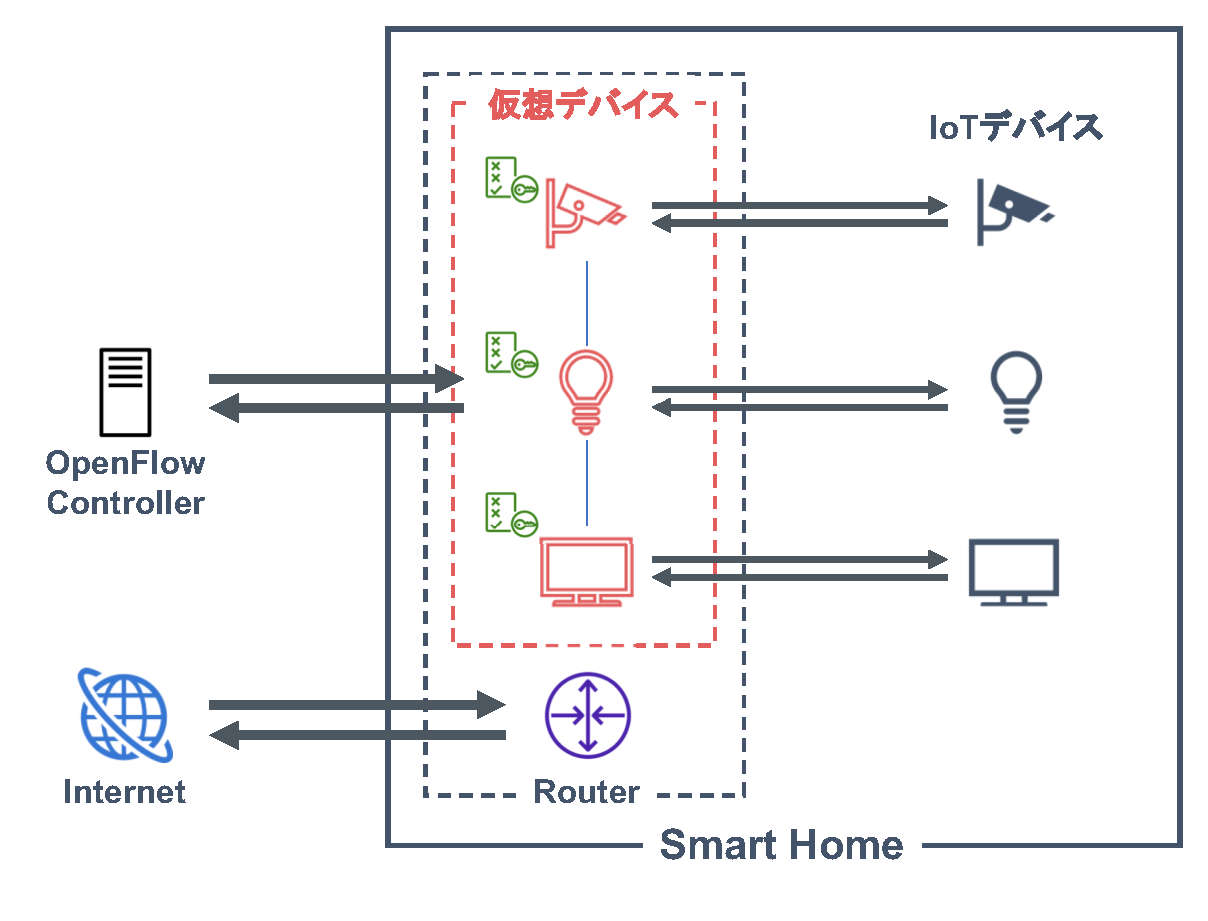
\includegraphics[width=\linewidth]{img/architecture.eps}
  \caption{提案システムの構成}
  \label{fig:architecture}
\end{figure}

% \begin{table*}[!bt]
%   \caption{IPAによるIoT高信頼化要件の定義}
%   \label{tab:IPA}
%   \centering
%   \begin{tabular}{c|l}
%     \hline
%     \multicolumn{2}{c}{IoT高信頼化要件}                                      \\
%     \hline \hline
%     開始 & [要件1]導入時や利用開始時に安全安心が確認できる                   \\
%     予防 & [要件2]稼働中の異常発生を未然に防止できる                         \\
%     検知 & [要件3]稼働中の異常発生を早期に検知できる                         \\
%     回復 & [要件4]異常が発生しても稼働の維持や早期の復旧ができる             \\
%     終了 & [要件5]利用の終了やシステム・サービス終了後も安心安全が確保できる \\
%     \hline
%   \end{tabular}
% \end{table*}

%---------------------------------------------------------------------
\section{提案システム}
\subsection{概要}
前述の問題点を受けて,IoTデバイス間通信における不正な通信の検知も必要である.
提案システムでは,SDNの代表的なプロトコルであるOpenFlowを利用することで,既存IoTデバイスや異なる規格などに対応でき,ホームネットワークに適した形で不正な通信の検知を実現する.
仮想デバイスというセキュリティ対策を適用可能なデバイスを,ゲートウェイ上に仮想的に作成する.ここにIoTデバイスがリソースの都合上適用できないセキュリティ対策をオフロードし,この仮想デバイスがIoTデバイスの通信を中継し,仮想デバイス間通信も可能にすることで,本来IoTデバイスに適用したいセキュリティ対策を実現する.
今回はセキュリティ対策として,ホームネットワーク内通信のトラフィック情報は既知であることを考慮し,フローの検証をOpenFlowコントローラ(OFC)で行う.


\subsection{システム構成}
OpenFlowを用いて,トラフィックフロー制御を行うことで,ホームネットワーク内で行われる通信を制限する.
提案システムの構成を\figref{fig:architecture}に示す.
構成要素としては,IoTデバイス,仮想デバイス,ルータ・ゲートウェイ,OFCから構成される.
IoTデバイスは,センサをはじめとした,リソースを十分に持たず,デバイスに直接セキュリティ対策を適用できないデバイスと定義する.
仮想デバイスは,IoTデバイスに要求されるセキュリティ対策を仮想的に実現したものである.IoTデバイスからの通信を中継し,セキュリティ対策を適用する.また,OpenFlowスイッチ(OFS)で構成し,仮想デバイス間通信を可能とする.OFSの機能を持った仮想デバイスをゲートウェイに配置し,OFCと通信を行うことでセキュリティ対策を実現する.


\begin{figure}[!tb]
  \centering
  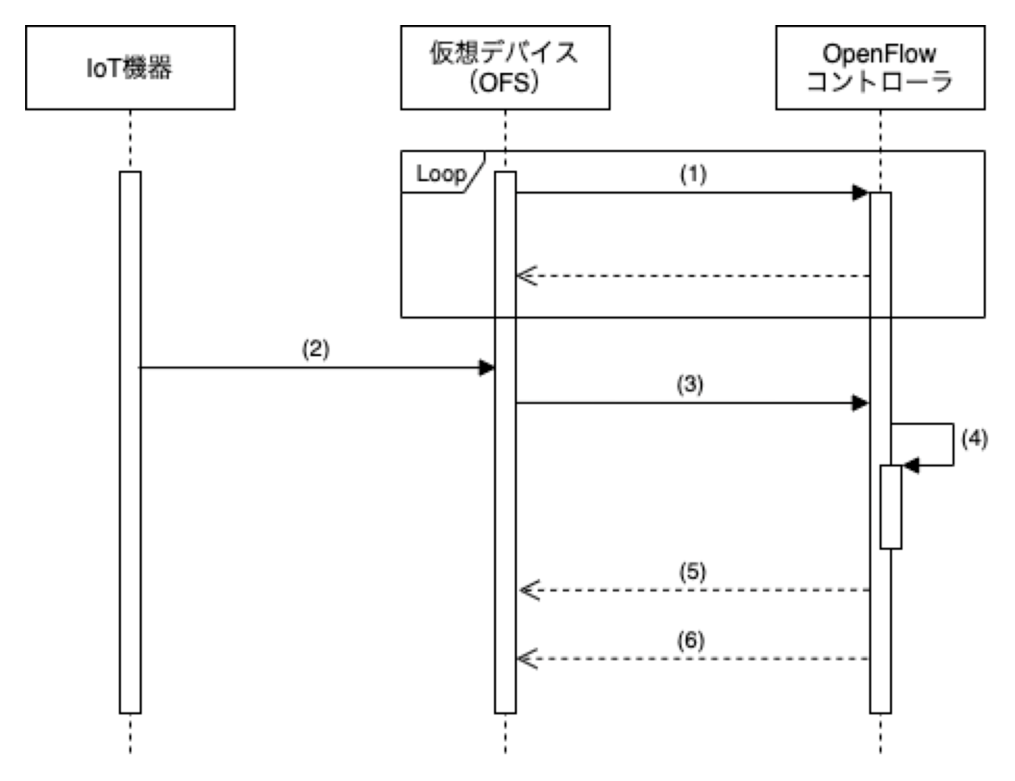
\includegraphics[width=\linewidth]{img/sequence.eps}
  \caption{提案システムの動作手順}
  \label{fig:sequence}
\end{figure}

\subsection{動作手順}
提案システムの動作手順を\figref{fig:sequence}に示し,詳細を以下に述べる.
送信先のIoTデバイスの仮想デバイスを仮想デバイスAとし,送信元のIoTデバイスの仮想デバイスを仮想デバイスBとする.

\begin{enumerate}
  \item ユーザは,OFCに仮想デバイスA作成要求
  \item OFCは,仮想デバイスAを作成
  \item 仮想デバイスAは,IoTデバイスを確認
  \item OFCと仮想デバイスAは互いに,Echo Request/Replyメッセージを定期的に送信
  \item 仮想デバイスBは,仮想デバイスAに通信
  \item 未知のフローだった場合,仮想デバイスAは,OFCに対してPacket Inメッセージを送信
  \item OFCは,トラフィック情報を調査
  \item OFCは,仮想デバイスAに対して許可/不許可メッセージとしてFlow Modメッセージを送信
  \item 仮想デバイスAは,フローを更新
  \item OFCは,仮想デバイスAに対してPacket Outメッセージを送信
\end{enumerate}

\subsection{想定環境}
ホームネットワークにおける閉じたデバイス間の通信,デバイス・クラウドサーバ通信,デバイス・ローカルサーバ通信を想定する.

%---------------------------------------------------------------------
\section{評価}
\subsection{評価項目}
本研究では,実用性と信頼性を評価する.
実用性では,システムの負荷がネットワークに与える影響を測定したいため,遅延を評価する.
信頼性では,IoTデバイスを用いたシステムの安心安全を確保するための機能として,IPAによりIoT高信頼化要件・機能要件が定義されている\cite{IPA}.本研究では,システムの稼働中の局面である予防,検知,回復の3つにおける高信頼化要件に対し,提案システムの有効性について考察する.


\subsection{評価シナリオ}
評価シナリオとしては,デバイス・クラウドサーバ通信,デバイス・ローカルサーバ通信を行っている状況を想定し,前述した関連研究との比較を行う.また,ルータ・ゲートウェイを経由したデバイス間通信の検証も行う.

%---------------------------------------------------------------------
\section{まとめ・今後の課題}
本研究では,ホームネットワークのセキュリティ上の課題として,十分なリソースを持たないIoTデバイスに起因するセキュリティ対策の困難さに着目した.
また,今後のスマートホームデバイスはデバイス間通信によって連携を行う形になることが想定される.
そこで本研究では,OpenFlowを用いてデバイス間通信における不正アクセスを軽減するシステムを提案した.
本提案システムでは,ルータ・ゲートウェイにOpenFlowスイッチの機能を持った仮想デバイスを配置し,トラフィック情報をOpenFlowコントローラで管理することで不正アクセスを防ぐ.実用性・信頼性を検証し,提案システムの有用性を示す.
今後は,トラフィックフロー調査によるセキュリティ対策の深堀りや評価シナリオの具体化を検討していく.

%---------------------------------------------------------------------
% Bibliography
\footnotesize{
  \begin{thebibliography}{99}
    \bibitem{guideline} IoT推進コンソーシアム, 総務省, 経済産業省, "IoTセキュリティガイドライン ver 1.0", 2016.
    \bibitem{logic} 今野裕太, 佐藤健哉, "論理デバイスプロキシを利用したIoTセキュリティプラットフォームの提案", 2017年度 情報処理学会関西支部 支部大会 講演論文集, Vol. 2017, 2017.
    \bibitem{d2d} C. Vallati et al., "Mobile-Edge Computing Come Home Connecting things in future smart homes using LTE device-to-device communications", IEEE Consumer Electronics Magazine, Vol.5, No.4, pp.77-83, 2016.
    \bibitem{disap} M. Serror et al., "Towards In-Network Security for Smart Homes", Proceedings of the 13th International Conference on Availability, Reliability and Security (ARES 2018), No.18, pp.1-8, 2018.
    \bibitem{IPA} IPA技術本部 ソフトウェア高信頼化センター(SEC), "「つながる世界の開発指針」の実践に向けた手引き", 2017.
    % \bibitem{OpenFlow} Nick McKeown et al., "OpenFlow: enabling innovation in campus networks", SIGCOMM Computer Communication Review, Vol.38, pp. 69–74, 2008.
  \end{thebibliography}
}

%---------------------------------------------------------------------
\end{document}
%---------------------------------------------------------------------
